\section{功}\label{sec:8-1}

在今后学习物理,以及学习其他科学技术知识的时候,经常要用到“功”这个词。
那么,什么叫“功” 呢?下面我们先看几个物理学中所说的做功的例子。

人推车前进的时候,人对车有一个向前的推力,车在力的作用下前进了一段距离。
物理学里就说,人对车做了功。

起重机吊起重物的时候,对重物有一个向上的拉力,重物在拉力的作用下升高了一段距离,
物理学里就说,起重机对重物做了功。

物理学里所说的\textbf{功包括两个必要的因素,一是作用在物体上的力,二是物体在力的方向上通过的距离}。

我们把砖托在手里不向上举,即使手臂累得发酸,也没有对砖做功。
这是因为砖虽然受到了托力,但并没有被托起一段距离。
我们推陷进泥地的汽车,如果没有把汽车推动,虽然累得筋疲力尽,还是没有对汽车做功。
可见物理学里说的做功,同日常生活里说的“做工”或“工作”含义是不同的。
在日常生活里,把一切消耗体力或脑力的劳动都说成是做工,含义很广;
而物理学里说的做功,含义要窄得多。

功的大小如何计算呢?

\begin{figure}[htbp]
    \centering
    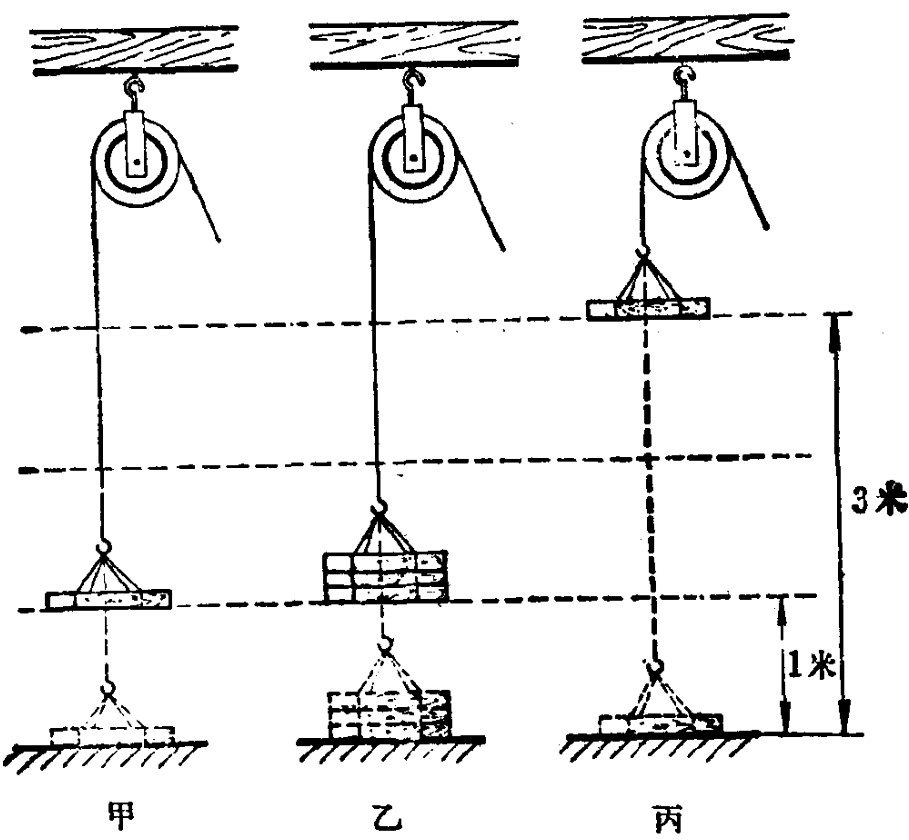
\includegraphics[width=0.6\textwidth]{../pic/czwl1-ch8-1}
    \caption{}\label{fig:8-1}
\end{figure}

把一块木板提高 1 米(图 \ref{fig:8-1} 甲),我们用了一定的力,做了一定量的功。
把三块木板提高 1 米〈图 \ref{fig:8-1} 乙),我们用了三倍的力,做了三倍的功。
把一块木板提高 3 米(图 \ref{fig:8-1} 丙),我们使木板通过了三倍的距离,也做了三倍的功。
可见,\CJKunderwave{功的大小跟作用在物体上的力成正比,还跟物体通过的距离成正比}。

物理学中规定:\textbf{功等于力跟物体在力的方向上通过的距离的乘积}。
$$ \textbf{功} = \textbf{力} \times \textbf{距离} \;\juhao $$

如果用 $F$ 表示力,$s$ 表示物体在力的方向上通过的距离,$W$ 表示功,上式可以写成
$$ W = Fs \;\juhao $$

在国际单位制中,力的单位是牛顿,距离的单位是米,功的单位就是牛顿·米,
牛顿·米有一个专门的名称叫做\text{焦耳}。
$$ 1 \jiaoer = 1 \niudunmi \;\juhao $$

在用公式 $W = Fs$ 计算功的时候,必须注意公式中的 $F$ 是作用在物体上的力,
$s$ 是物体在力 $F$ 作用下沿力的方向通过的距离。
例如,在平路上拉着一辆重 1500 牛顿的车前进了 10 米,就不能说这时做的功是重力乘以距离,
即 $1500 \niudun \times 10 \mi = 15\;000 \jiaoer$。
因为重力的方向向下,车并没有在它的作用下向下移动,而是沿水平方向移动了 10 米。
只有测出水平方向的拉力才能计算出我们做了多少功。
如果测出这个拉力是 100 牛顿,那么正确的答案应该是
$$ W = Fs = 100\niudun \times 10\mi = 1000\jiaoer \;\juhao$$


\lianxi

(1) 一个小孩用力提一桶水,但是没有把桶提起来,他做功了吗?

(2) 我们把重 1000 牛顿的箱子沿着水平地板推动 1 米,我们所做的功是不是等于 1000 焦耳?
为什么?要计算推箱子所做的功,还必须知道什么?

(3) 工人把质量为 10 千克的一张桌子,搬到 10 米高的楼上去,工人所做的功是多少?

(4) 为了给一个工厂供水,每天需要用水泵把 $300\lfm$ 的水送到 40 米高的地方。水泵所做的功是多少?

(5) 马拉着质量是 2000 千克的车在平路上前进了 400 米,做了 $3 \times 10^5$ 焦耳的功,求马的水平拉力是多少牛顿。


